\documentclass[conference,letterpaper]{IEEEtran}
\usepackage[T1]{fontenc}
\usepackage{amsmath,amssymb}
\usepackage{graphicx}
\usepackage{booktabs}
\usepackage{multirow}
\usepackage{cite}
\usepackage{url}
\usepackage{xcolor}
\usepackage[hidelinks]{hyperref}

\setlength{\textfloatsep}{5pt plus 1.5pt minus 1.5pt}
\setlength{\dbltextfloatsep}{6pt plus 1.5pt minus 1.5pt}
\setlength{\floatsep}{4pt plus 1pt minus 1pt}
\setlength{\abovecaptionskip}{2pt}
\setlength{\belowcaptionskip}{0pt}

\newcommand{\pp}{\ensuremath{\,\mathrm{pp}}}
\newcommand{\Hwhole}{\mathcal{H}_{\mathrm{whole}}}
\newcommand{\Hagree}{\mathcal{H}_{\mathrm{agree}}}
\newcommand{\Hslot}{\mathcal{H}_{\mathrm{slot}}}
\newcommand{\SymBiPhrase}{\textsc{SymBiPhrase}}
\newcommand{\SymBiList}{\textsc{SymBiList}}
\newcommand{\crc}{\textsc{CRC}}

\newcommand{\pl}{\smash{$^\ddagger$}}
\newcommand{\sig}{\smash{$^\dagger$}}

\title{Symmetric Agreement-Anchored Phrase Recombination\\for Frozen Multilingual ASR}

\author{\IEEEauthorblockN{Zhifan Pan\textsuperscript{1,2,3},
Yingxiong Gao\textsuperscript{1,2,3},
Maihemuti Maimaiti\textsuperscript{1,2,3,*},
Yifeng Yu\textsuperscript{1,2,3}, Aishan Wumaier\textsuperscript{1,2,3}}
\IEEEauthorblockA{\textsuperscript{1}School of Computer Science and Technology, Xinjiang University, Urumqi, China\\
\textsuperscript{2}Xinjiang Multimodal Intelligent Processing and Information Security\\
Engineering Technology Research Center, Xinjiang University, Urumqi, China\\
\textsuperscript{3}Joint International Research Laboratory of Silk Road Multilingual\\
Cognitive Computing, Xinjiang University, Urumqi, China\\
\textsuperscript{*}Corresponding author: mahmutjan@xju.edu.cn}}

\begin{document}
\maketitle

\begin{abstract}
Frozen multilingual speech recognizers frequently produce complementary local transcriptions across languages and architectures, yet post-decoding fusion faces a \emph{granularity--asymmetry trade-off}: whole-hypothesis reranking cannot recombine complementary phrases, whereas word-level voting or arbitrary cuts shatter donor phrases under recognizer asymmetry. We propose \SymBiList{}, a zero-hallucination, millisecond-latency phrase recombination framework requiring neither acoustic fine-tuning, word timestamps, nor speech resynthesis. Aligning scored $N$-best lists to an anchor grid and fixing unanimously agreed words induces a phrase space ($\Hwhole \subseteq \Hagree \subseteq \Hslot$) that preserves intact donor phrases. To eliminate single-anchor bias, we run dedicated directional models in both anchor orientations and reconcile residual disagreements via an anti-symmetric Pass-2 block arbiter (\SymBiPhrase{}). We further replace pointwise trees with a lightweight neural listwise expected-edit ranker over 32d block-context features and introduce Conformal Risk-Controlled Deferral (\crc{}) for finite-sample harm guarantees. Across FLEURS-12 and cross-corpus Kathbath (valid and unseen-speaker test), \SymBiList{} reaches 21.67\%, 35.24\%, and 36.41\% macro WER (5.55\%, 6.77\%, 7.16\% CER) in 3.0~ms/utterance CPU, outperforming whole-list controls on all 12 languages, fixed-length cuts even without Amharic, MBR, ROVER, and confusion networks; scaling to 3-system CTC+CTC+AED fusion lowers FLEURS-12 further to 21.50\% WER / 5.51\% CER. On an untouched 8-language Common Voice 26 CTC+AED benchmark (7 unseen languages), symmetric recombination cuts WER by 3.52\pp{} below the best single model and transfers zero-shot ($-2.05\pp$ on unseen languages). Code is available at \href{https://github.com/Zhifan-Pan/symbilist-asr}{\nolinkurl{github.com/Zhifan-Pan/symbilist-asr}}.
\end{abstract}

\begin{IEEEkeywords}
multilingual speech recognition, system combination, phrase recombination, listwise ranking, conformal risk control
\end{IEEEkeywords}

\section{Introduction}
Frozen multilingual automatic speech recognition (ASR) foundation models—both non-autoregressive connectionist temporal classification (CTC) encoders such as MMS~\cite{pratap2024mms}, OWSM-CTC~\cite{peng2024owsmctc}, and Omnilingual ASR~\cite{omni2025}, and autoregressive encoder--decoder (AED) models such as Whisper~\cite{radford2023whisper}—exhibit strong complementarity across languages, scripts, and error modes. Post-decoding combination avoids costly multi-encoder retraining, yet exposes a structural dilemma: whole-hypothesis reranking~\cite{yan2025reranking} preserves fluency without hallucination but cannot recombine local phrases; word voting and confusion networks~\cite{fiscus1997rover,mangu2000consensus,benes2024hystoc} allow word-level edits but sever phrase dependencies and inflate insertions under word-boundary mismatch; and LLM generative error correction (GER)~\cite{chen2023hyporadise,ma2025correction,yang2025covoger} incurs high latency and hallucination risk~\cite{hu2024listen}.

We investigate three questions: \textbf{RQ1:} \emph{Which boundaries govern effective multilingual phrase recombination?} \textbf{RQ2:} \emph{How does anchor orientation bias affect fusion under recognizer asymmetry, and can bidirectional symmetry neutralize it?} \textbf{RQ3:} \emph{Can listwise block ranking and distribution-free risk control compress the oracle--selection gap while bounding harm?}

Our analysis reveals a \emph{granularity--asymmetry mechanism}. When an anchor splits morphological affixes—as in FLEURS Amharic (49.95\% anchor WER vs.\ 27.31\% donor WER despite 6.47\% anchor CER)—fixed-length or slot partitions slice donor words on the fragmented grid, doubling insertions. Fixing only unanimously agreed words keeps donor phrases intact across disagreement spans, while dedicated bidirectional reconciliation eliminates single-anchor bias without scrambling anchor-relative deltas.

We contribute: (1) a \textbf{formal agreement phrase space} ($\Hwhole \subseteq \Hagree \subseteq \Hslot$) with zero-hallucination support and pure boundary-position controls ($Q_{\mathrm{var}}, Q_{\mathrm{shift}}$); (2) \textbf{symmetric bidirectional reconciliation (\SymBiPhrase{})} neutralizing anchor bias across CTC+CTC and CTC+AED pairs; (3) \textbf{listwise expected-edit ranking (\SymBiList{}) and Conformal Risk Control (\crc{})} compressing selection error at 3.0~ms/utterance CPU with finite-sample harm ceilings; and (4) \textbf{multilingual, cross-architecture, and unseen-language validation} across FLEURS-12, Kathbath valid/test, 3-system fusion, and untouched Common Voice 26 (7 unseen languages).

\section{Related Work}
\emph{Voting, confusion networks, and MBR.} Classical ROVER~\cite{fiscus1997rover}, LM-weighted voting~\cite{schwenk2000combining}, and confusion networks (CN)~\cite{mangu2000consensus} merge aligned words; Hystoc~\cite{benes2024hystoc} extracts lattice-free word confidences from end-to-end $N$-best lists. Minimum Bayes Risk (MBR) decoding minimizes expected risk, with recent progress in model-based MBR~\cite{jinnai2024mbmbr}, low-rank factorization~\cite{trabelsi2024lowrankmbr}, and uncertainty-aware abstention~\cite{daheim2025uambr}. Our block expected edit-distance features act as block-decomposed dual-source MBR risks that naturally factor pairwise comparisons into small disagreement blocks.

\emph{Segment recombination, reranking, and LLM-GER.} READ~\cite{li2026read} uses text and timestamp agreement to form segments scored via pretrained TTS acoustic discrepancy; our approach requires neither timestamps nor TTS and runs in 3~ms CPU. Multilingual $N$-best reranking~\cite{yan2025reranking} stays limited to $\Hwhole$, while LLM-GER frameworks—HyPoradise~\cite{chen2023hyporadise}, CoVoGER~\cite{yang2025covoger}, UADF~\cite{chen2024uadf}, Listen-Again~\cite{hu2024listen}, and TASLP GER~\cite{ma2025correction}—enable open rewriting at higher latency and hallucination risk. DualHyp~\cite{kim2024dualhyp} highlights dual-stream reliability routing, motivating our symmetric arbiter (Table~\ref{tab:related}).

\emph{Multilingual metrics and risk control.} Normalization and word segmentation heavily affect multilingual WER relative to CER~\cite{manohar2024normalization,thomas2025cer}, while subword/phonetic cues aid low-resource transfer~\cite{yusuyin2024whistle}. Motivated by pairwise/listwise ensembling~\cite{jiang2023llmblender} and Conformal Risk Control~\cite{angelopoulos2024crc}, we jointly optimize WER/CER via listwise block ranking and distribution-free harm deferral.

\begin{table}[t]
\caption{Positioning of \SymBiList{} vs.\ representative ASR fusion paradigms.}\label{tab:related}
\centering\scriptsize\setlength{\tabcolsep}{1.8pt}\renewcommand{\arraystretch}{0.94}
\begin{tabular*}{\columnwidth}{@{\extracolsep{\fill}}lccccc@{}}\toprule
Paradigm & Recomb. & 0-Hallu. & No TTS & Multi-Lang & ms\\\midrule
ROVER/Hystoc~\cite{fiscus1997rover,benes2024hystoc} & Word & $\checkmark$ & $\checkmark$ & $\checkmark$ & $<$5\\
Whole Rerank~\cite{yan2025reranking} & None & $\checkmark$ & $\checkmark$ & $\checkmark$ & $<$5\\
READ~\cite{li2026read} & Segment & $\checkmark$ & $\times$ & Limited & $>$500\\
LLM-GER~\cite{ma2025correction,yang2025covoger} & Free Gen. & $\times$ & $\checkmark$ & Partial & $>$200$^\dagger$\\
\textbf{\SymBiList{} (Ours)} & \textbf{Sym.\ Phr.} & $\checkmark$ & $\checkmark$ & $\checkmark$ & \textbf{3.0}\\
\bottomrule
\multicolumn{6}{l}{\tiny $^\dagger$GPU decoding (1B--7B autoregressive models); others measured on CPU.}
\end{tabular*}
\end{table}

\begin{figure*}[t]
\centering
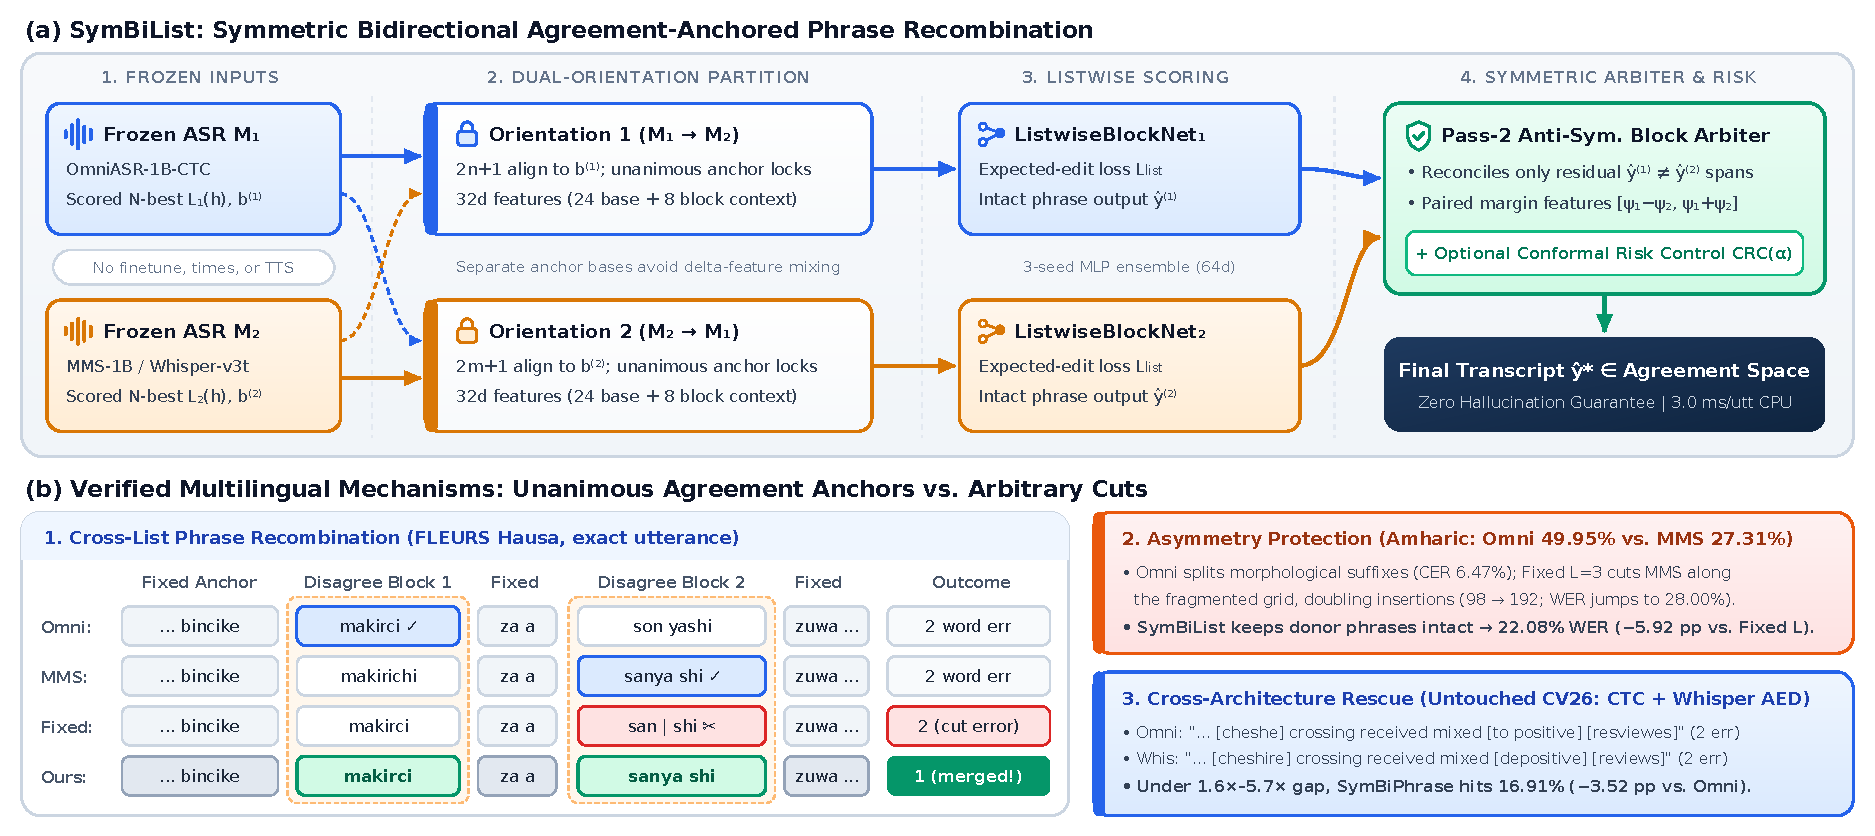
\includegraphics[width=0.82\textwidth]{figures/method_overview.pdf}
\caption{Overview of \SymBiList{} and verified multilingual mechanisms. (a) Dual-orientation agreement partitioning builds separate anchor bases ($M_1{\to}M_2$, $M_2{\to}M_1$) fed to dedicated directional \texttt{ListwiseBlockNet} scorers; an anti-symmetric Pass-2 arbiter reconciles residual disagreements with optional Conformal Risk Control (\crc{}). (b) Verified examples showing cross-list phrase recovery (Hausa), suffix-split asymmetry protection (Amharic), and cross-architecture CTC+AED rescue (CV26 English).}
\label{fig:method}
\vspace{-6pt}
\end{figure*}

\section{Proposed Method}
\subsection{Candidate Alignment and Agreement Phrase Space}
Given $S \ge 2$ frozen recognizers $\{M_1,\dots,M_S\}$, each source $s$ supplies a greedy transcript $b^{(s)}$ and scored $N$-best list $\mathcal{L}_s=\{(h, L_s(h))\}$. Strings undergo deterministic Unicode normalization (NFC, lowercase, NFC, Unicode punctuation replaced by spaces, whitespace collapsed, combining marks retained). Equal normalized strings within source $s$ merge via log-sum-exp, giving conditional masses
\begin{equation}
p_s(h)=\frac{\exp(L_s(h)/T)}{\sum_{h'\in\mathcal{L}_s}\exp(L_s(h')/T)},\qquad T=0.5.
\label{eq:mass}
\end{equation}

Fix anchor $b = (w_1,\dots,w_n)$. Every $h \in \Hwhole = \bigcup_{s=1}^S \mathcal{L}_s$ aligns to $b$ by unit word Levenshtein distance (tie order: diagonal, deletion, insertion), giving a lossless projection $\pi_b(h)$ over $2n{+}1$ cells ($n$ word cells $\{1,3,\dots,2n{-}1\}$ and $n{+}1$ gap cells $\{0,2,\dots,2n\}$; $\mathrm{read}(\pi_b(h))=h$). Word cell $2i{-}1$ is \emph{fixed} iff every retained hypothesis projects $w_i$ there:
\begin{equation}
\mathcal{F}_b = \big\{2i{-}1 : \forall h \in \Hwhole,\; \pi_b(h)_{2i-1} = w_i\big\}.
\end{equation}
Maximal contiguous runs of non-fixed cells form variable blocks $B_1,\dots,B_K$. Block $j$ admits the distinct intact phrases $V_j$ read from complete projections across $B_j$, with anchor phrase $v_{j,0}$ first.

\emph{Proposition 1 (Containment and Zero-Hallucination Support).} Let $\Hagree=\{\bigoplus_{j=1}^K v_j : v_j \in V_j\}$ interleaved with fixed anchor words, and let $\Hslot$ be the cell-level Cartesian product. Then: (i) $\Hwhole \subseteq \Hagree \subseteq \Hslot$; (ii) every emitted word occurs in some $h \in \Hwhole$; and (iii) every local phrase $v_j \in V_j$ occurs contiguously in some $h \in \Hwhole$. \emph{Proof:} Lossless projection maps each $h \in \Hwhole$ to $v_j(h)=\mathrm{read}(\pi_b(h)_{B_j}) \in V_j$, so $h \in \Hagree$; intact-substring admissibility restricts $\Hslot$ and forbids out-of-list vocabulary.\hfill$\square$

\subsection{Block Features and Intra-Block Competition Context}
For candidate $v \in V_j$, let $y = b[v_{j,0} \leftarrow v]$ be the single-block replacement and $A = \max(1, |b|_w)$. Table~\ref{tab:features} specifies all 32 target-free features (24 base + 8 intra-block competition context). A Witten--Bell character 4-gram LM (spaces/EOS retained, additive-0.1 unigrams) and word bigram LM ($c/(c{+}t)$ interpolation) fit solely on training transcripts supply length- and anchor-normalized char4 deltas
\begin{equation}
F_\mu(y)=\frac{\ell(y)}{|y|+1}-\frac{\ell(b)}{|b|+1},\quad
F_\Sigma(y)=\frac{\ell(y)-\ell(b)}{|b|+1},
\label{eq:lm}
\end{equation}
plus word2 deltas. Projecting $p_s$ into block $j$ yields $P_{s,j}$ and local expected edit-risk deltas for $k\in\{w,c\}$:
\begin{equation}
R_{s,j}^{(k)}(v)=\frac{1}{A_k}\sum_{a\in V_j} P_{s,j}(a)\big[d_k(v,a)-d_k(v_{j,0},a)\big].
\label{eq:risk}
\end{equation}
To expose within-block competition to neural/tree scorers, we append 8 zero-cost context features (within-$V_j$ $z$-scores and gaps to the block best for $F_\Sigma$, word2 per-char delta, $R_{1,j}^{(w)}$, and $R_{2,j}^{(w)}$, plus cross-source mass entropy).

\begin{table}[t]
\caption{32-dimensional block-candidate feature schema (24d base + 8d context).}\label{tab:features}
\centering\scriptsize\setlength{\tabcolsep}{1.8pt}\renewcommand{\arraystretch}{0.94}
\begin{tabular*}{\columnwidth}{@{\extracolsep{\fill}}lcl@{}}\toprule
Family & Dim & Constituents (Anchor-Relative / Target-Free)\\\midrule
Edit Geometry & 7 & Anc--Don div., cell pos., $|V_j|$, $|v|_w$, $|v_0|_w$, $d_w/A$, $\Delta|v|_c$\\
Char 4-gram LM & 2 & Per-char delta $F_\mu(y)$, anchor-norm sum delta $F_\Sigma(y)$\\
Word 2-gram LM & 3 & Per-tok delta, per-char delta, $\Delta$OOV fraction\\
Source Dist./Risk & $6S$ & $P_{s,j}(v)$, $P_{s,j}(v_0)$, $|\mathrm{supp}|$, $\max P_{s,j}$, $R_{s,j}^{(w)}$, $R_{s,j}^{(c)}$\\
Block Context & 8 & Within-$V_j$ $z$-score \& best-gap (LM, risk), mass entropy\\
\bottomrule\end{tabular*}
\end{table}

\subsection{Listwise Ranking, Bidirectional Symmetry, and CRC Deferral}
\emph{Differentiable Listwise Expected-Edit Ranker (\texttt{ListwiseBlockNet}).} Let $\Delta e_j^{(w)}(v), \Delta e_j^{(c)}(v)$ be language-length-normalized edit changes on the training fold. Pointwise squared-error trees waste capacity fitting absolute errors of irrelevant suboptimal options. We instead train a 2-layer residual MLP $f_\theta(x_{j,v})\in\mathbb{R}^2$ (64 hidden units, LayerNorm, SiLU, dropout 0.15; 3-seed ensemble) directly on block-level expected edit loss:
\begin{equation}
\mathcal{L}_{\mathrm{list}}(\theta)=\sum_{j}\omega_j\Big[\sum_{v\in V_j}q_\theta(v|B_j)\tilde{e}_j(v)+\beta\,\mathrm{KL}(q_\theta\|q^*)\Big],
\label{eq:listwise}
\end{equation}
where $q_\theta(v|B_j)$ is the softmax of $-s_\theta(v)/\tau_r$ over $V_j$ with $s_\theta(v)=\hat{z}_w(v)+\alpha_c\hat{z}_c(v)$ ($s_\theta(v_{j,0})\equiv 0$), $\tilde{e}_j(v)=\Delta e_j^{(w)}(v)+\alpha_c\Delta e_j^{(c)}(v)$, $q^*$ is the soft target over $V_j$, $\beta{=}0.2$, and $\omega_j$ equalizes language weights.

\emph{Symmetric Bidirectional Reconciliation (\SymBiPhrase{} / \SymBiList{}).} Fixing $M_1$ as anchor biases alignment whenever $M_2$ outperforms $M_1$, yet switching anchors inside one regressor degrades accuracy by mixing anchor-delta bases (Section~\ref{sec:ablation}). We instead fit dedicated directional scorers $f^{(1)}$ ($M_1{\to}M_2$) and $f^{(2)}$ ($M_2{\to}M_1$) producing $\hat{y}^{(1)}, \hat{y}^{(2)}$, align them by exact agreement, and resolve only residual spans $(u_1,u_2)$ via an out-of-fold Pass-2 anti-symmetric arbiter $g([\psi(u_1){-}\psi(u_2),\,\psi(u_1){+}\psi(u_2)])$ over Pass-1 margins, LM deltas, and source risks (Fig.~\ref{fig:method}a). Since $\hat{y}^{(1)},\hat{y}^{(2)}\in\Hagree$, Proposition~1 holds verbatim.

\emph{Conformal Risk-Controlled Deferral (\crc{}).} Let $y_{\mathrm{whole}}$ be the best whole hypothesis under the same scorer and $m(x){=}S(y_{\mathrm{whole}}){-}S(\hat{y}^*)\ge 0$ the recombination margin. For rule $\hat{y}_\lambda = \hat{y}^*$ if $m(x)\ge\lambda$ else $y_{\mathrm{whole}}$, harm $H_i(\lambda)=\mathbb{I}[d_w(\hat{y}_\lambda,r_i)>d_w(y_{\mathrm{whole}},r_i)]$ is monotonically non-increasing in $\lambda$. Conformal Risk Control~\cite{angelopoulos2024crc} calibrates on held-out folds:
\begin{equation}
\hat{\lambda}(\alpha) = \inf\Big\{\lambda \ge 0 : \frac{1+\sum_{i=1}^{n_{\mathrm{cal}}} H_i(\lambda)}{n_{\mathrm{cal}}+1} \le \alpha\Big\},
\label{eq:crc}
\end{equation}
guaranteeing $\mathbb{E}[H_{\mathrm{test}}(\hat{\lambda})] \le \alpha$ for exchangeable utterances at any harm ceiling $\alpha$. \emph{Complexity:} Running both directional alignments ($\mathcal{O}(SNL_w^2)$ for sentence length $L_w$), 32d feature extraction, 3-seed MLP inference, Pass-2 reconciliation, and optional \crc{} deferral requires 3.0~ms/utterance on CPU.

\section{Experimental Setup}
\emph{Models and Benchmarks.} We evaluate homogeneous CTC+CTC, heterogeneous CTC+AED, and 3-system fusion across three benchmarks: (1) \textbf{FLEURS-12 Dev}~\cite{conneau2023fleurs}: 4,078 recordings across 12 languages (\texttt{am, hy, ast, bn, ka, ha, he, kea, kn, ckb, ta, uk}) with 32,940 train transcripts solely for Char4/Word2 LMs. CTC+CTC pairs \texttt{omniASR\_CTC\_1B\_v2}~\cite{omni2025} with \texttt{facebook/mms-1b-all}~\cite{pratap2024mms} (closed 12-route \texttt{mms-lid-126}, 4-beam exact CTC rescoring); Stage-2A adds \texttt{openai/whisper-large-v3-turbo} (4-beam FP16 AED). (2) \textbf{Kathbath Valid \& Test}~\cite{javed2023indic}: 4,920 validation (2,770 \texttt{ta}, 2,150 \texttt{kn}; 40 speakers) and 3,030 unseen-speaker \texttt{clean/testunk} utterances (40 disjoint speakers), evaluated strictly zero-target-label from FLEURS-12 fits. We distinguish originally sealed locked baseline test readouts from our \emph{post-lock} evaluation of the frozen FLEURS-12 \SymBiList{} checkpoint. (3) \textbf{Untouched Common Voice 26}~\cite{ardila2020commonvoice}: 2,000 crowdsourced utterances (250/lang) across 1 seen (\texttt{ta}) and \textbf{7 unseen languages} (\texttt{ar, tr, sw, ru, gl, es, en}) pairing \texttt{omniASR\_CTC\_1B\_v2} with \texttt{whisper-large-v3-turbo} (unrestricted auto-LID), under \textbf{Protocol Z1} (strictly zero-shot from FLEURS-12, zero CV26 labels/LM) and \textbf{Protocol Z3} (5-fold OOF with train-fold text LM).

\emph{Baselines, Controls, and Statistical Testing.} All comparators consume identical scored lists: unsupervised Hystoc--ROVER~\cite{benes2024hystoc,fiscus1997rover}, Exact N-best MBR~\cite{jinnai2024mbmbr}, zero-supervision Agreement Block-MBR; supervised Calibrated word CN, \emph{Whole (refit/fixed)}, \emph{Learned word slots} ($\Hslot$); and boundary controls \emph{Fixed} ($F, L{=}3$), \emph{Matched random} ($Q$, 5 seeds), plus pure-position controls $Q_{\mathrm{var}}$ (matching exact per-utterance variable-block counts) and $Q_{\mathrm{shift}}$ ($\pm 2$-cell shifts). Primary metrics are macro WER and nonspace Unicode CER across three prompt-group-disjoint 5-fold splits (seeds 17, 42, 2026) with inner-fold $\alpha_c \in \{0.5,1.0\}$. Following~\cite{dror2018significance}, we compute paired cluster bootstrap 95\% CIs (10,000--50,000 draws; prompt groups on FLEURS, speakers on Kathbath, utterances on CV26).

\begin{table*}[t]
\caption{Main CTC+CTC results (OmniASR-1B-CTC + MMS-1B-all) on FLEURS-12 dev (3 grouped splits), Kathbath valid (cross-corpus), and Kathbath clean/testunk (unseen speakers). Bold marks best scored system; $\dagger$ denotes 95\% paired cluster CI strictly $<0$ vs.\ Agree A and Whole (fixed).}\label{tab:main}
\centering\scriptsize\setlength{\tabcolsep}{3.0pt}\renewcommand{\arraystretch}{0.84}
\begin{tabular*}{\textwidth}{@{\extracolsep{\fill}}llccccccr@{}}\toprule
& & \multicolumn{2}{c}{\textbf{FLEURS-12 Dev (4,078)}} & \multicolumn{2}{c}{\textbf{Kathbath Valid (4,920)}} & \multicolumn{2}{c}{\textbf{Kathbath Test (3,030)}} & \\
\cmidrule(lr){3-4}\cmidrule(lr){5-6}\cmidrule(lr){7-8}
Group & Method & WER (\%) $\downarrow$ & CER (\%) $\downarrow$ & WER (\%) $\downarrow$ & CER (\%) $\downarrow$ & WER (\%) $\downarrow$ & CER (\%) $\downarrow$ & WERR$^*$\\\midrule
\multirow{2}{*}{Single}
& Anchor greedy (OmniASR) & 27.400 & 6.245 & 38.773 & 7.342 & 39.487 & 7.734 & 0.0\%\\
& Donor greedy (MMS) & 27.852 & 6.928 & 42.082 & 8.089 & 43.439 & 8.577 & $-1.6$\%\\\midrule
\multirow{4}{*}{Unsup.}
& Hystoc--ROVER~\cite{benes2024hystoc,fiscus1997rover}\pl & 27.588 & 8.008 & 39.175 & 9.842 & 40.274 & 10.306 & $-0.7$\%\\
& Exact MBR (word, whole)\pl & 26.391 & 6.335 & 38.581 & 7.392 & 39.454 & 7.797 & +3.7\%\\
& Block MBR (word, agree)\pl & 26.148 & 6.261 & 38.409 & 7.331 & 39.265 & 7.752 & +4.6\%\\
& Exact MBR + Char4 LM\pl & 23.668 & 5.914 & 36.889 & 7.034 & 37.871 & 7.436 & +13.6\%\\\midrule
\multirow{7}{*}{Sup.\ Ctrl}
& Calibrated word CN & 23.246 & 7.792 & 36.234 & 9.405 & 37.089 & 9.861 & +15.2\%\\
& Whole (refitted HGB) & 22.946{\tiny$\pm$.043} & 5.833 & 36.468 & 6.938 & 37.430 & 7.306 & +16.3\%\\
& Whole (fixed HGB costs) & 22.722{\tiny$\pm$.017} & 5.811 & 36.315 & 6.952 & 37.356 & 7.346 & +17.1\%\\
& Whole (fixed Listwise)\pl & 22.692{\tiny$\pm$.023} & 5.758 & 36.067 & 6.905 & 37.164 & 7.295 & +17.2\%\\
& Learned word slots ($\Hslot$) & 22.525{\tiny$\pm$.016} & 6.627 & 35.691 & 7.593 & 36.566 & 8.059 & +17.8\%\\
& Random partition ($Q$)\pl & 22.369 & 6.292 & 35.751 & 7.418 & 36.735 & 7.843 & +18.4\%\\
& Fixed length ($F, L{=}3$)\pl & 22.264 & 6.360 & 35.542 & 7.509 & 36.433 & 8.033 & +18.7\%\\\midrule
\multirow{4}{*}{\textbf{Ours}}
& Agree Phrase A (Omni anc., HGB) & 21.948{\tiny$\pm$.037} & 5.631 & 35.725 & 6.840 & 36.805 & 7.283 & +19.9\%\\
& Agree Phrase A0 (MMS anc., HGB)\pl & 21.893{\tiny$\pm$.061} & 5.591 & 35.567 & 6.811 & 36.680 & 7.227 & +20.1\%\\
& \SymBiPhrase{} (HGB, 24d)\pl & 21.738{\tiny$\pm$.084} & 5.588 & 35.354 & 6.792 & 36.565 & 7.225 & +20.7\%\\
& \textbf{\SymBiList{} (32d Listwise)}\pl & \textbf{21.672}{\tiny$\pm$.030}\sig & \textbf{5.552}\sig & \textbf{35.236}\sig & \textbf{6.772}\sig & \textbf{36.409}\sig & \textbf{7.161}\sig & \textbf{+20.9\%}\\\midrule
\multirow{2}{*}{\textcolor{gray}{\emph{Oracle}}}
& \textcolor{gray}{\emph{Whole list oracle ($\Hwhole$)}} & \textcolor{gray}{\emph{19.569}} & \textcolor{gray}{\emph{4.892}} & \textcolor{gray}{\emph{30.667}} & \textcolor{gray}{\emph{5.814}} & \textcolor{gray}{\emph{31.800}} & \textcolor{gray}{\emph{6.217}} & \textcolor{gray}{\emph{+28.6\%}}\\
& \textcolor{gray}{\emph{Agreement phrase oracle ($\Hagree$)}} & \textcolor{gray}{\emph{17.318}} & \textcolor{gray}{\emph{4.331}} & \textcolor{gray}{\emph{28.750}} & \textcolor{gray}{\emph{5.369}} & \textcolor{gray}{\emph{29.915}} & \textcolor{gray}{\emph{5.775}} & \textcolor{gray}{\emph{+36.8\%}}\\
\bottomrule
\multicolumn{9}{l}{\tiny $^*$FLEURS WERR vs.\ OmniASR (27.400\%). $^\ddagger$Post-lock clean/testunk readouts of frozen FLEURS-12 fits (unmarked test rows: sealed baselines; \SymBiList{} 3.03~ms/utt CPU).}
\end{tabular*}
\end{table*}

\begin{figure*}[t]
\centering
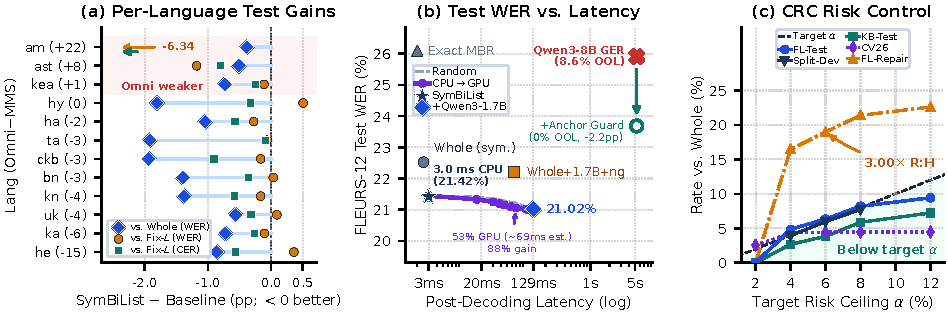
\includegraphics[width=0.86\textwidth]{figures/mechanism_and_risk.pdf}
\caption{Scientific mechanisms on FLEURS-12 and Kathbath. (a) Per-language $\Delta$WER and $\Delta$CER vs.\ Fixed-$L$ ($F$), ordered by Anchor$-$Donor WER asymmetry: agreement protects weak-anchor languages (\texttt{am\_et}, \texttt{ast\_es}), while \SymBiList{} wins 12/12 CER and improves non-Amharic mean WER ($-0.11\pp$). (b) Support vs.\ Selection Gap plane (dotted lines mark constant Actual$-$Oracle gap): finer partitions inflate selection error whereas \SymBiList{} compresses it directly. (c) Conformal Risk Control (\crc{}) keeps empirical harm strictly below $\alpha$ on FLEURS and cross-corpus Kathbath.}
\label{fig:mechanism}
\vspace{-4pt}
\end{figure*}

\section{Results and Analysis}
\subsection{Main CTC+CTC Results and Post-Lock Test Verification}
Table~\ref{tab:main} shows three clear findings. First, with \emph{zero supervision or LM}, Agreement Block-MBR (26.148\%/6.261\% FLEURS; 38.409\%/7.331\% Kathbath) beats Whole Exact MBR (26.391\%/6.335\%; 38.581\%/7.392\%) on every metric, proving structural value prior to learning. Second, \SymBiList{} resolves every prior weakness of unidirectional Agreement (A): bidirectional symmetry (\SymBiPhrase{}) cuts WER from 21.948\%/35.725\% to 21.738\%/35.354\% (95\% CI vs.\ A: $[-0.389,-0.208]\pp$ FLEURS; $[-0.523,-0.273]\pp$ Kathbath), and 32d listwise ranking (\SymBiList{}) reaches \textbf{21.672\% / 5.552\%} on FLEURS and \textbf{35.236\% / 6.772\%} on Kathbath—beating \emph{every} baseline including Fixed-$L$ (35.542\%) and Slots (35.691\%) on both WER and CER (\texttt{kn\_in} 30.03\%/6.09\%, \texttt{ta\_in} 40.44\%/7.45\%). On FLEURS, \SymBiList{} beats \emph{Whole (fixed)} on \textbf{12/12 languages} (Amharic: 22.08\% vs.\ 22.58\%), beats A on \textbf{11/12 languages}, and beats Fixed-$L$ even excluding Amharic ($-0.108\pp$ mean across the other 11 languages, 12/12 CER wins). Under the \emph{identical} listwise scorer (\emph{Whole fixed Listwise}: 22.692\%/36.067\%), phrase recombination isolates pure gains of \textbf{$-1.020\pp$ FLEURS} and \textbf{$-0.831\pp$ Kathbath}. Third, on unseen-speaker Kathbath \texttt{clean/testunk}, the frozen FLEURS-12 \SymBiList{} achieves \textbf{36.409\% WER / 7.161\% CER} in \textbf{3.03~ms/utterance} CPU (9.18~s total), with 95\% CIs strictly $<0$ vs.\ A ($-0.396$ $[-0.601,-0.184]$ WER; $-0.122$ $[-0.157,-0.089]$ CER), \emph{Whole (refit)} ($-1.021$ $[-1.317,-0.718]$ WER; $-0.146$ $[-0.188,-0.104]$ CER), and \emph{Whole (fixed)} ($-0.947$ $[-1.168,-0.719]$ WER), while posting lower WER and $-0.899\pp$ $[-1.068,-0.741]$ lower CER than \emph{Slots} (36.566\%/8.059\%).

\subsection{Cross-Architecture (CTC+AED), Unseen Languages, and 3-Way Fusion}
Table~\ref{tab:stage2} reports untouched Common Voice 26 cross-architecture fusion (\texttt{OmniASR-1B-CTC} + \texttt{Whisper-large-v3-turbo}) and Stage-2A FLEURS/Kathbath CTC+AED and 3-system results. On CV26, Whisper excels on high-resource languages (\texttt{ru} 5.7\%, \texttt{es} 5.8\%, \texttt{en} 9.6\%, \texttt{tr} 19.4\% vs.\ OmniASR 12.9\%, 9.2\%, 16.4\%, 26.7\%) but suffers unrestricted auto-LID collapse on \texttt{sw} (105.3\%) and \texttt{ta} (67.5\%) where OmniASR gets 18.6\% and 37.1\%. Unsupervised voting/MBR collapses (33.8--34.9\%) and unidirectional A exhibits strong anchor lock-in (18.651\% Omni-anc.\ vs.\ 17.572\% Whisper-anc., hurting \texttt{ta} to 40.0\%).

Under \textbf{Protocol Z1} (strictly zero-shot from FLEURS-12, zero CV26 labels/LM), listwise scoring transfers strongly, slashing Unseen-7 WER from 18.047\% to \textbf{15.886\%} (Listwise Omni-anc.) and \textbf{15.993\%} (\SymBiList{}; All-8 19.412\%, $-1.02\pp$ All-8, $-2.05\pp$ Unseen-7), whereas zero-shot HGB degrades (21.712\%). Under \textbf{Protocol Z3} (5-fold OOF), \SymBiPhrase{} (HGB) reaches \textbf{16.912\% / 4.927\%} All-8 (\textbf{13.994\% / 4.863\%} Unseen-7), beating OmniASR by \textbf{$-3.517\pp$} (17.2\% WERR), unidirectional A by $-1.739\pp$, \emph{Whole (fixed HGB)} by $-1.889\pp$, Fixed-$L$ by $-1.891\pp$, and \emph{Slots} by $-0.751\pp$. Under CV26's extreme 1.6$\times$--5.7$\times$ dominance gap, restricting \texttt{ListwiseBlockNet} to whole sentences (\emph{Listwise Whole fixed}: 16.744\%) edges out \SymBiList{} (17.029\%, $\Delta{=}{+}0.285$ $[+0.012,+0.574]$), driven by \texttt{ta} (37.9\% vs.\ 38.6\%) where Whisper emits wrong-language text—clarifying that phrase switching thrives under complementary parity while single-model collapse favors whole-sentence deferral.

\emph{Stage-2A FLEURS/Kathbath CTC+AED \& 3-System ($S{=}3$).} On FLEURS-12, Whisper auto-LID averages 93.177\% WER across all 12 low-resource languages (86.529\% Kathbath), yet fusing it with OmniASR or MMS via \SymBiPhrase{}/\SymBiList{} safely extracts $-1.94\pp$ (\texttt{Omni+Whis} 25.459\%/5.949\%) and $-3.17\pp$ (\texttt{MMS+Whis} 24.683\%/6.367\%) below the CTC model without noise corruption ($-2.05\pp$ to $-4.13\pp$ on the 9 Whisper-native FLEURS languages). Scaling to 3 heterogeneous systems (\texttt{Omni+MMS+Whis}, 38d features), \textbf{3-Way \SymBiList{}} sets our best overall FLEURS-12 result at \textbf{21.498\% WER / 5.508\% CER} (+21.5\% WERR; $-0.448\pp$ $[-0.614,-0.294]$ vs.\ \emph{3-Way Whole Listwise} 21.947\%, $-0.781\pp$ vs.\ \emph{3-Way Phrase HGB} 22.279\%, $-1.298\pp$ vs.\ \emph{3-Way Whole HGB} 22.796\%), while also beating all 3-way baselines on Kathbath WER (35.900\% vs.\ 36.364\%--36.820\%; 95\% CIs strictly $<0$).

\begin{table}[t]
\caption{Cross-architecture (CTC+AED) on Common Voice 26 (5-fold OOF) and Stage-2A FLEURS/Kathbath 3-system fusion (grouped 5-fold, seed 17).}\label{tab:stage2}
\centering\scriptsize\setlength{\tabcolsep}{1.7pt}\renewcommand{\arraystretch}{0.84}
\begin{tabular*}{\columnwidth}{@{\extracolsep{\fill}}lcccc@{}}\toprule
& \multicolumn{2}{c}{\textbf{CV26 All-8}} & \multicolumn{2}{c}{\textbf{CV26 Unseen-7}}\\
\cmidrule(lr){2-3}\cmidrule(lr){4-5}
Method (OmniASR-CTC + Whisper-AED) & WER $\downarrow$ & CER $\downarrow$ & WER $\downarrow$ & CER $\downarrow$\\\midrule
OmniASR-CTC (greedy) & 20.429 & 5.914 & 18.047 & 6.031\\
Whisper-v3t (AED, auto-LID) & 35.880 & 15.244 & 31.362 & 15.175\\
Unsup.\ Block MBR & 33.802 & 14.570 & 30.071 & 14.636\\\midrule
\multicolumn{5}{l}{\emph{Protocol Z1: Strictly Zero-Shot (FLEURS-12 fit, 0 CV26 labels/LM)}}\\
Z1 Phrase A (HGB, Omni anc.) & 21.712 & 6.282 & 18.187 & 6.195\\
Z1 Listwise (Omni anc.) & 19.574 & 5.730 & \textbf{15.886} & \textbf{5.552}\\
Z1 \SymBiList{} (Zero-Shot) & \textbf{19.412} & 5.744 & 15.993 & 5.622\\\midrule
\multicolumn{5}{l}{\emph{Protocol Z3: CV26 5-Fold OOF (train-fold text LM)}}\\
Whole (fixed HGB) & 18.801 & 5.490 & 16.269 & 5.545\\
Learned word slots (HGB) & 17.663 & 5.832 & 15.035 & 5.798\\
Unidir.\ A (Omni anc.) & 18.651 & 5.444 & 16.114 & 5.490\\
Unidir.\ A (Whis anc.) & 17.572 & 5.194 & 14.364 & 5.088\\
\textbf{\SymBiPhrase{} (HGB, Ours)} & \textbf{16.912} & \textbf{4.927} & 13.994 & \textbf{4.863}\\
\SymBiList{} (32d Listwise, Ours) & 17.029 & 5.005 & \textbf{13.952} & 4.889\\
\emph{Listwise Whole (fixed, ref.)} & \emph{16.744} & \emph{4.900} & \emph{13.726} & \emph{4.827}\\\midrule
& \multicolumn{2}{c}{\textbf{FLEURS-12}} & \multicolumn{2}{c}{\textbf{Kathbath Valid}}\\
\cmidrule(lr){2-3}\cmidrule(lr){4-5}
\emph{Stage-2A: CTC+AED \& 3-System ($S{=}3$)} & WER $\downarrow$ & CER $\downarrow$ & WER $\downarrow$ & CER $\downarrow$\\\midrule
Omni+Whis: Whole (HGB) & 26.053 & 6.047 & 37.438 & 7.208\\
Omni+Whis: \SymBiPhrase{} (HGB) & 25.459 & 5.949 & 37.249 & 7.212\\
MMS+Whis: Whole (HGB) & 25.040 & 6.393 & 40.481 & 7.929\\
MMS+Whis: \SymBiPhrase{} (HGB) & 24.683 & 6.367 & 40.567 & 8.035\\
3-Way (O+M+W): Whole (HGB) & 22.796 & 5.768 & 36.820 & 7.008\\
3-Way: Phrase (HGB) & 22.279 & 5.660 & 36.505 & \textbf{6.960}\\
3-Way: Whole (Listwise) & 21.947 & 5.628 & 36.364 & 6.987\\
\textbf{3-Way \SymBiList{} (Ours)} & \textbf{21.498} & \textbf{5.508} & \textbf{35.900} & 6.974\\
\bottomrule\end{tabular*}
\end{table}

\subsection{Ablations, Boundary Isolation, and Risk Control}\label{sec:ablation}
Table~\ref{tab:ablation} consolidates five diagnostic studies on identical FLEURS-12 and Kathbath splits. \emph{Features \& importance:} Removing all LMs raises WER by $+3.15\pp$ (FLEURS) and $+2.57\pp$ (Kathbath); removing source distributions/risks raises WER by $+0.27\pp$/$+0.17\pp$. Permutation importance reveals cross-corpus LM differentiation: \texttt{char4\_delta\_norm\_sum} surges from $+1.172\pp$ (FLEURS) to $+1.705\pp$ (Kathbath), while \texttt{word2\_delta\_per\_char} drops from $+0.996\pp$ to $+0.340\pp$, showing why character $n$-grams transfer across agglutinative morphology~\cite{yusuyin2024whistle}; donor risk (\texttt{src2\_exp\_word\_risk}: $+0.293\pp$/$+0.331\pp$) ranks right behind LMs. \emph{Boundary placement:} Matching decision counts strictly ($Q_{\mathrm{var}}$, 2.73 var.\ blocks) or shifting boundaries by $\pm 2$ cells ($Q_{\mathrm{shift}}$) degrades all four metrics (22.472/5.944 and 22.245/6.146 FLEURS; 36.062/7.133 and 35.780/7.404 Kathbath), isolating boundary placement from block count. \emph{Anchor \& scorer:} Mixed-base \emph{DynAnchor} degrades (21.989\%/35.806\%), soft agreement ($\tau{=}0.90$) trades Kathbath WER for CER ($+0.036\pp$), while HGB-24d $\to$ Pairwise-32d $\to$ Unidir.\ Listwise $\to$ \SymBiList{} improves monotonically on both corpora. \emph{Data \& temperature:} Only 10\% of training prompt groups ($\approx$27 utt/lang) already beats 100\%-trained \emph{Whole} and \emph{CN}; $T \in [0.25, 2.0]$ is stable around $T{=}0.5$, whereas uniform $T{\to}\infty$ degrades (22.024\%/35.786\%).

\emph{Mechanism \& \crc{} safety.} Fig.~\ref{fig:mechanism}(a) shows agreement protecting weak-anchor languages (\texttt{am\_et} $+22.6\pp$, \texttt{ast\_es} $+8.9\pp$) where Fixed-$L$ slices MMS words on OmniASR's suffix-split grid (Amharic insertions double 98$\to$192, WER 28.00\% vs.\ \SymBiList{} 22.08\%) while winning 12/12 CER. Fig.~\ref{fig:mechanism}(b) maps the Support--Selection law: finer spaces lower DP oracle WER (19.57\%$\to$16.34\%) yet inflate selection error (3.15$\to$6.19\pp), whereas \SymBiList{} compresses selection error vertically to 4.35\pp{} FLEURS and 6.49\pp{} Kathbath. Fig.~\ref{fig:mechanism}(c) confirms \crc{} holds empirical harm $\hat{R}_{\mathrm{emp}} \le \alpha$ for every $\alpha \in \{0.02,\dots,0.12\}$ on FLEURS (0.016--0.090) and zero-recalibration Kathbath (0.010--0.070), achieving a 5.2$\times$ repair-to-harm ratio (331 vs.\ 64) at $\alpha{=}0.02$.

\begin{table}[t]
\caption{Unified ablations on FLEURS-12 dev \& Kathbath valid (3-seed means; identical candidate lists and splits).}\label{tab:ablation}
\centering\scriptsize\setlength{\tabcolsep}{1.8pt}\renewcommand{\arraystretch}{0.86}
\begin{tabular*}{\columnwidth}{@{\extracolsep{\fill}}lrrrr@{}}\toprule
& \multicolumn{2}{c}{\textbf{FLEURS-12}} & \multicolumn{2}{c}{\textbf{Kathbath}}\\
Variant & WER $\downarrow$ & CER $\downarrow$ & WER $\downarrow$ & CER $\downarrow$\\\midrule
\emph{Base Unidir.\ A (HGB 24d)} & 21.948 & 5.631 & 35.725 & 6.840\\\midrule
\multicolumn{5}{l}{\emph{4-Family Feature Ablations (on Base A)}}\\
\quad w/o Edit Geometry (17d) & 21.989 & 5.649 & 35.669 & 6.829\\
\quad w/o Source Dist./Risk (12d) & 22.222 & 5.671 & 35.895 & 6.891\\
\quad w/o Word 2-gram LM (21d) & 22.683 & 5.724 & 35.807 & 6.874\\
\quad w/o Char 4-gram LM (22d) & 22.668 & 5.761 & 36.997 & 7.038\\
\quad w/o All Text LMs (19d) & 25.097 & 6.191 & 38.295 & 7.352\\\midrule
\multicolumn{5}{l}{\emph{Pure Boundary Placement \& Anchor Controls}}\\
\quad $Q_{\mathrm{var}}$ (decision-matched) & 22.472 & 5.944 & 36.062 & 7.133\\
\quad $Q_{\mathrm{shift}}$ ($\pm 2$-cell shift) & 22.245 & 6.146 & 35.780 & 7.404\\
\quad DynAnchor (mixed-base HGB) & 21.989 & 5.650 & 35.806 & 6.846\\
\quad Soft Agree ($\tau{=}0.90$) & 21.935 & 5.656 & 35.599 & 6.876\\\midrule
\multicolumn{5}{l}{\emph{Scorer Architecture \& Symmetry Progression}}\\
\quad MLP + 32d Block Context & 21.874 & 5.577 & 35.418 & 6.781\\
\quad Pairwise HGB + 32d Context & 21.793 & 5.573 & 35.338 & 6.782\\
\quad Unidir.\ Listwise (32d) & 21.736 & 5.559 & 35.293 & 6.771\\
\quad \textbf{\SymBiList{} (Bidir.\ Listwise)} & \textbf{21.672} & \textbf{5.552} & \textbf{35.236} & \textbf{6.772}\\\midrule
\multicolumn{5}{l}{\emph{Data Efficiency \& Temperature $T$ (on Base A)}}\\
\quad 10\% / 25\% train groups & 22.27/22.07 & 5.67/5.65 & 36.00/35.82 & 6.96/6.89\\
\quad $T{=}0.25$ / $T{\to}\infty$ (uniform) & 21.94/22.02 & 5.63/5.64 & 35.74/35.79 & 6.86/6.86\\
\bottomrule\end{tabular*}
\end{table}

\section{Discussion, Limitations, and Conclusion}
\emph{Utility and scope.} Because acoustic encoders stay frozen, \SymBiList{} adds only 3.0~ms/utterance CPU post-processing (RTF $<5{\times}10^{-4}$), zero GPU memory, and strict zero-hallucination support—ideal for multilingual pseudo-labeling and edge/batch ASR fusion. Three limitations bound our claims: (1) \SymBiList{} on Kathbath \texttt{clean/testunk} is a frozen \emph{post-lock} evaluation (Common Voice 26 provides our untouched external test); (2) under catastrophic single-model LID collapse (CV26 \texttt{ta}/\texttt{sw}), whole-sentence listwise deferral can beat cross-block switching; and (3) training optimizes edit distance rather than semantic fidelity, leaving acoustic uncertainty and open-set LID integration for future work.

\emph{Conclusion.} We presented \SymBiList{}, combining unanimous agreement-anchored phrase boundaries, anti-symmetric bidirectional reconciliation, 32d listwise expected-edit ranking, and Conformal Risk-Controlled Deferral. Across FLEURS-12, Kathbath valid/test, 3-system fusion, and untouched 8-language Common Voice 26 (CTC+AED, 7 unseen languages), it resolves the granularity--asymmetry trade-off in 3.0~ms/utt CPU with verified zero-hallucination support.

\section*{Acknowledgment}
Supported by NSFC Grant 62466058 and the Autonomous Region Key R\&D Program Grant 2025B03042-1.

\renewcommand{\IEEEbibitemsep}{0pt plus 0.2pt}
\bibliographystyle{IEEEtran}
\bibliography{references}
\end{document}
